\chapter{Noisy Softplus: an Activation Function Enables Training Deep SNNs Off-line as ANNs}
\label{cha:Conv}
%Paragraph One: LINK
The first step in answering my research question of validating the capability of real-time cognitive application built on neuromorphic platform was to build an object recognition prototype running completely on hardware in an absolute spike-based fashion.
It built up the basis for the later research that neuromorphic hardware has been capable of running large cognitive applications standing alone without a general computer and has stepped into the era of improving its cognitive ability.
It is also possible to make a link between this chapter and the whole argument that this work contributes to an effective SNN training method equivalent to the performance of ANN's.

%Paragraph Two: FOCUS
%Now focus the reader’s attention on what this chapter is specifically going to do and why it is important. In this chapter I will examine.. I will present… I will report … This is crucial in (aim of thesis/research question) in order to….
The Spiking Neural Network (SNN) has not achieved the recognition/classification performance of its non-spiking competitor, the ANN, particularly when used in deep neural networks.
Training SNNs by conventional ANN algorithms and mapping well-trained ANNs weights to SNNs are attracting attention in this field for its straight-forward conception.
%, especially the SNNs of spiking neurons with biological characteristics.
In this chapter we will propose a new biologically-inspired activation function, Noisy Softplus, which is well-matched to the response function of LIF (Leaky Integrate-and-Fire) neurons.
Thus, any ANN employing Noisy Softplus neurons, even of deep architecture, can be trained exactly by the traditional algorithm (e.g. Back Propagation) and the trained weights can easily fit into the spiking version of the same network.
This is crucial to increase the classification accuracy of SNNs using biological characteristics and close the gap between the performance of SNNs and ANNs.

%Paragraph Three: OVERVIEW
%The third paragraph simply outlines the way that you are going to achieve the aim spelled out in the previous paragraph. It’s really just a statement of the contents in the order that the reader will encounter them. It is important to state these not simply as topics, but actually how they build up the internal chapter argument… I will begin by examining the definitions of, then move to seeing how these were applied… I first of all explain my orientation to the research process, positioning myself as a critical scholar.. I then explain the methodology that I used in the research, arguing that ethnography was the most suitable approach to provide answers to the question of… 
%https://patthomson.net/2014/01/16/connecting-chapterschapter-introductions/

%We first of all explore the research question of on-line, event-based deep SNN training in the literature.
%We then describe SRM in mathematical expression, and explain the factors influencing the accuracy of the method and the factors not. 
%Afterwards we argue why the learning algorithm is proper to train spiking Autoencoders (SAEs) and Spiking Restricted Boltzmann Machines (SRBM).
%During the research we encountered the problem introduced by the correlated spikes, therefore we also propose solutions to decorrelate spike trains in Section~\ref{sec:problem}. 
%Finally the detailed comparison of the traditional training and SRM learning on MNIST dataset demonstrates the equivalent learning ability and shows similar even surpassing recognition and reconstruction capability of SAE and SRBM.
We begin by introducing the difficulty of SNN training, and lead to the existing solutions state-of-the-art.
Then we put forward the proposed activation function, Noisy Softplus, and demonstrate how it fits the network dynamics of SNNs.
The complete SNN training method is explained employing the new activation function.
To validate the classification accuracy, a convolutional network (ConvNet) is trained on the MNIST database following this training mechanism and tested directly on an SNN.
The encouraging result demonstrates the equivalent recognition capability of the more biologically-realistic SNNs and bring biological features to the activation units in ANNs.

\section{Introduction}	
Deep Neural Networks (DNNs) are the most promising research field in computer vision, even exceeding human-level performance on image classification tasks~\cite{he2015delving}.
To investigate whether brains might work similarly on vision tasks, these powerful DNN models have been converted to spiking neural networks (SNNs).
In addition, the spiking DNN offers the prospect of neuromorphic systems that combine remarkable performance with energy-efficient training and operation.

Theoretical studies have shown that biologically-plausible learning, e.g. Spike-Timing-Dependent Plasticity (STDP), could approximate a stochastic version of powerful machine learning algorithms
%	~\cite{nessler2013bayesian,neftci2013event,neftci2013event,o2016deep}.
such as 
%	Expectation Maximization~\cite{nessler2013bayesian}, 
Contrastive Divergence~\cite{neftci2013event}, Markov Chain Monte Carlo~\cite{buesing2011neural} and Gradient Descent~\cite{o2016deep}.
Stochasticity, in contrast with the continuously differentiable functions used by ANNs, is intrinsic to the event-based spiking process, making network training difficult.
In practice, ANNs use neuron and synapse models very different from biological neurons, and it remains an unsolved problem to develop SNNs with equivalent performance.

%How to map a well trained ANN to SNN is a hot topic in this field, especially using spiking neurons of biological scale.

Conversely, the offline training of an ANN, which is then mapped to an SNN, has shown near loss-less conversion and state-of-the-art classification accuracy.
This research aims to prove that SNNs are equally capable as their non-spiking rivals of pattern recognition, and at the same time are more biologically realistic and energy-efficient.
Jug et. al.~\cite{Jug_etal_2012} first proposed the use of the Siegert function to replace the sigmoid activation function in Restricted Boltzmann Machine (RBM) training.
The Siegert units map incoming currents driven by Poisson spike trains to the response firing rate of a Leaky Integrate-and-Fire (LIF) neuron.
The ratio of the spiking rate to its maximum is equivalent to the output of a sigmoid neuron.
A spiking Deep Belief Network (DBN)~\cite{Stromatias2015scalable} was implemented on neuromorphic hardware, SpiNNaker~\cite{furber2014spinnaker}, to recognise hand written digits in real time.
However, cortical neurons seldom saturate their firing rate.
Thus Rectified Linear Units (ReLU) were proposed and surpassed the performance of other popular activation units thanks to their advantage of sparsity~\cite{glorot2011deep} and its robustness towards the vanishing gradient problem which will be described in Section~\ref{sec:activation}.
%TODO Chapter2 about relu and vanishing gradient problem.
%	~\cite{dugas2001incorporating}.
%trained with noisy input, the 4-layered spiking autoencoder reached 98.37\% accuracy on MNIST. 

Even better performance~\cite{cao2015spiking,diehl2015fast} has been demonstrated in Spiking Convolutional Networks (ConvNets), but this employed simple integrate and fire (IF) neurons.
The training used only ReLUs and zero bias to avoid negative outputs, and applied a deep learning technique, dropout, to increase the classification accuracy.
Normalising the trained weights for use on an SNN was relatively straightforward and maintained the classification accuracy.
This work was extended to a Recursive Neural Network (RNN)~\cite{diehl2016conversion} and run on the TrueNorth~\cite{merolla2014million} neuromorphic hardware platform.


	
\section{Modelling The Activation Function}

\subsection{Neural Science Background}
	%As discussed above, most of the top scored networks map the ReLUs in ANN to the equivalent spiking version of IF neurons.
	This paper proposes a new activation function, Noisy Softplus, which is inspired by neuroscience observations of LIF neurons.
	The LIF neuron model follows the following membrane potential dynamics:
	\begin{equation}
	\tau_m \frac{\D V}{\D t}=V_{rest} - V + R_{m} I(t) ~.
	\label{eq:LIF_V}
	\end{equation}
	The membrane potential $V$ changes in response to the input current $I$, starting at the resting membrane potential $V_{rest}$, where the membrane time constant is $\tau_m = R_mC_m$, $R_m$ is the membrane resistance and $C_m$ is the membrane capacitance.
	The central idea in converting spiking neurons to activation units lies in the response function of a neuron model.
	Given a constant current injection $I$, the response function, i.e. firing rate, of the LIF neuron is:
	\begin{equation}
	\lambda_\mathit{out}=
	\left [ t_\mathit{ref}-\tau_m\log \left ( 1-\frac{V_{th}-V_\mathit{rest}}{IR_m}  \right )\right ]^{-1}, \textrm{~when~} IR_m>V_{th}-V_{rest},
	\label{equ:consI}
	\end{equation}
	otherwise the membrane potential cannot reach the threshold $V_{th}$ and the output firing rate is zero. 
	The absolute refractory period $t_\mathit{ref}$ is included, where all input during this period is ignored.
	The dotted (zero noise) line in Figure~\ref{Fig:physics} illustrates the response function of an LIF neuron, which inspired the proposal of ReLUs.
	The parameters of the LIF neuron are all biologically valid (see the listed values in Table~\ref{tbl:pynnSetting}), and the same parameters are used throughout this paper.
	In practice, a noisy current generated by the arrival of spike trains, rather than a constant current, flows into the neurons.
	The response function~\cite{la2008response}	of the LIF neuron to a noisy current is as follows, where $\mu$ and $\sigma$ are the mean and variance of the current:
	\begin{equation}
	\lambda_\mathit{out}=
	\left [ t_\mathit{ref}+\tau_m \int_{\frac{V_\mathit{rest}-\mu \tau_m }{\sigma \sqrt{\tau_m}}}^{\frac{V_{th}-\mu \tau_m }{\sigma \sqrt{\tau_m}}} \sqrt{\pi} \exp(u^{2}) (1+erf(u)) \D u \right ]^{-1} ~.
	\label{equ:noiseI}
	\end{equation}
	
	\begin{figure}
		\centering
		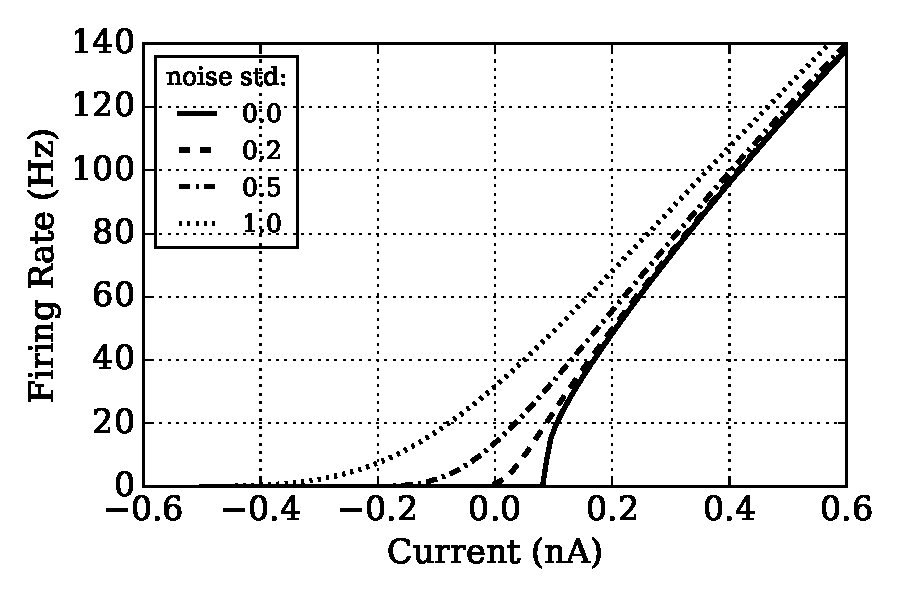
\includegraphics[width=0.6\textwidth]{pics_iconip/1.pdf}
		\caption{Response function of the LIF neuron with noisy input currents with different standard deviations.}
		\label{Fig:physics}
	\end{figure}
	
	\begin{table}[bt]
		\centering
		\caption{\label{tbl:pynnConfig}Parameter setting for the current-based LIF neurons using PyNN.}
		\bgroup
		\def\arraystretch{1.4}
		\begin{tabular}{c c c}
					%\hline
					Parameters & Values & Units \\
					\hline
					cm & 0.25 & nF	\\
					%\hline
					tau\_m & 20.0 & ms\\
					%\hline
					tau\_refrac & 1.0 & ms\\
					%\hline
					tau\_syn\_E & 5.0 & ms\\
					%  %\hline
					tau\_syn\_I & 5.0 & ms\\
					%  %\hline
					v\_reset & -65.0 & mV\\
					%\hline
					v\_rest & -65.0 & mV\\
					%\hline
					v\_thresh & -50.0 & mV\\
					%\hline
					i\_offset & 0.1 & nA\\
			\hline
%			Parameters & cm & tau\_m & tau\_refrac & tau\_syn\_E & tau\_syn\_I & v\_rest & v\_thresh & i\_offset \\
%			Values & 0.25 &  20.0 & 1.0 & 5.0 & 5.0 & -65.0 & -50.0  & 0.1 \\
%			Units & nF & ms & ms & ms & ms & mV & mV& nA\\
%			\hline
		\end{tabular}
		\egroup
	\end{table}

	\subsection{Activation Function in ANN}
	\label{sec:activation}
	Nair and Hinton~\cite{nair2010rectified} stated that ReLU preserve information about relative intensities(intensity equivarance) provided they have zero biases and are noise-free, but binary units do not.
	This technique has dominated the best recognition performances~\textcolor{red}{ref?} in deep learning.
	Furthermore, utilising ReLU in SNNs will simplify the network structure significantly because of the zero biases.
	Thus in this section we firstly demonstrate on how ReLU work and perform in DBN.
	
	The input vector in a ReLU based RBM does no longer have to be binary, so it can be a float.
	Instead of using sigmoid transfer function, the ReLU is always positive and has no upper boundary.
	There are three different ways to model ReLU~\ref{Fig:relu_tranf}:
	\begin{figure}[hbt]
		\centering
		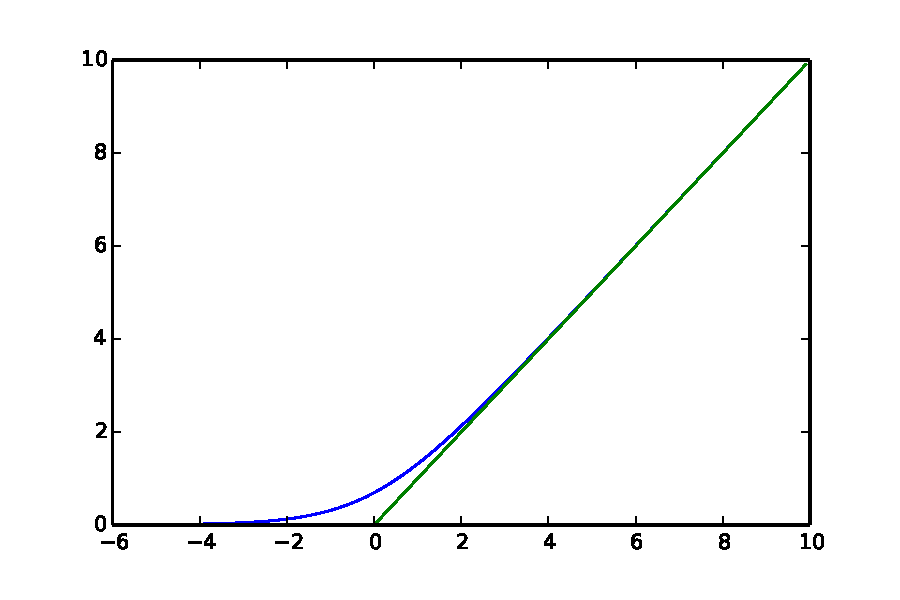
\includegraphics[width=0.7\textwidth]{pics_sdbn/relu.pdf}
		\caption{The DBN architecture.} 
		\label{Fig:relu_tranf}
	\end{figure}
	\begin{itemize}
		\item sum of an infinite number of binary units with each having a bias less than the previous one~~\cite{nair2010rectified}.
		This is one of the reason people believe the recognition performance exceeding since each ReLU represents infinite samples of sigmoid. 
		\item the approximation of the previous form $\log(1+e_x)$.
		\item the simplified version which is the most popular in deep learning $max(0,\sum w x)$.
	\end{itemize}  
	
	Recent work~\cite{hunsberger2015spiking} proposed the Soft LIF response function, which is equivalent to Softplus activation.
	
	
	\subsection{LIF Neuron Simulation}
	To verify the response function, a simulation was carried out using PyNN~\cite{davison2008pynn} to compare with the analytical results.
	A noisy current with a particular $\mu$ and $\sigma$ was injected into an LIF neuron for 10~s.
	The firing rate was the average among 10 trials, see Figure~\ref{Fig:lif_curr}.
	The slight difference compared to the analytical results (dashed lines) comes from the time resolution of the simulated noisy current.
	
	\begin{figure}
		\centering
		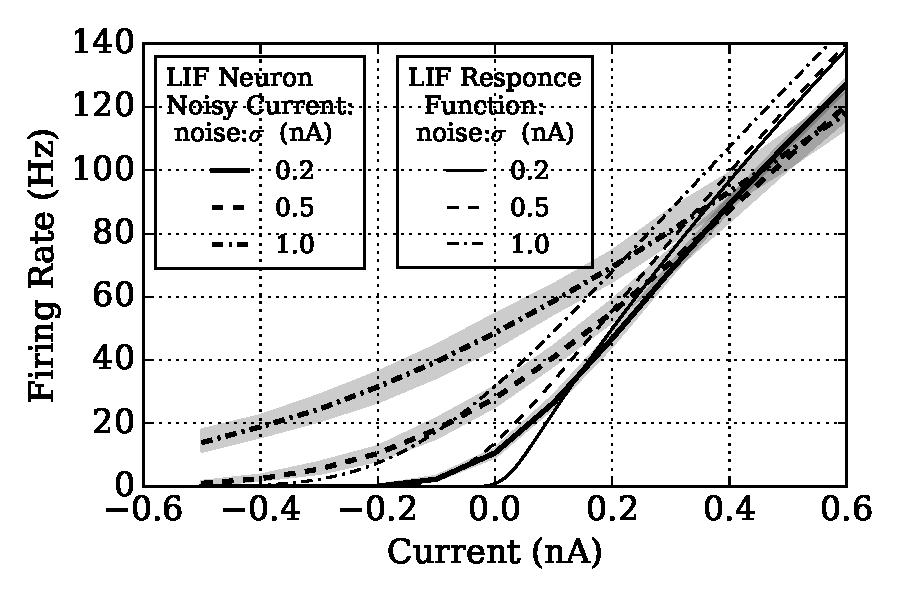
\includegraphics[width=0.6\textwidth]{pics_iconip/2.pdf}
		\caption{Comparing the recorded firing rates of the LIF neuron simulation driven by noisy currents to the response function shown in Figure~\ref{Fig:physics}.}
		\label{Fig:lif_curr}
	\end{figure}
	
	A more realistic simulation of a noisy current is generated by a Poisson spike train, 
	%assuming that large amount of small amplitude PSPs are required to reach the threshold and $\tau_syn$ limits to 0.
	where the mean and variance are given by:
	\begin{equation}
	\mu = \tau_{syn}\sum_i w_i\lambda_{i}~,~\sigma^2=\frac{1}{2}\tau_{syn}\sum_i w_i^2\lambda_{i}~,
	\end{equation}
	where $\tau_{syn}$ is the synaptic time constant, and each Poisson spike train connects to the neuron with a strength of $w_i$ and a firing rate of $\lambda_i$.
	Two populations of Poisson spike sources, for excitatory and inhibitory synapses respectively, were connected to a single LIF neuron to mimic the noisy currents.
	The firing rates of the Poisson spike generators were determined by the given $\mu$ and $\sigma$.
	Figure~\ref{Fig:lif_pois} illustrates the recorded firing rates responding to the spike trains compared to the result driven by noisy currents.
	The use of noisy currents assumes that the post-synaptic potential (PSP) is a delta function, e.g. $\tau_{syn}$ tends to the limits of 0.
	However, in practice the release of neurotransmitter takes time and the noise added to the mean current is not pure white noise.
	Thus we observe a slight mismatch with the test of the noisy current. %todo rephrase
%	Thus the experiments show that a longer $\tau_{syn}$ increases the level of noise and widens the variance of the output firing rate.
	\begin{figure}
		\centering
		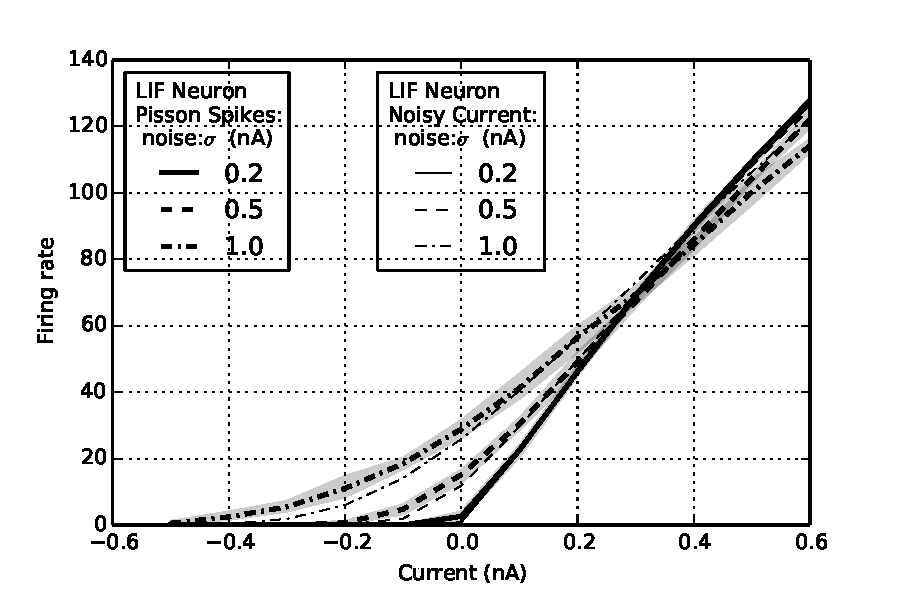
\includegraphics[width=0.6\textwidth]{pics_iconip/3-1.pdf}
		\caption{Recorded response firing rate of a LIF neuron.
			The driving noisy current is simulated with Poission spike trains and the results are compared to the noisy current source.}
		\label{Fig:lif_pois}
	\end{figure}	
%	\begin{figure}[bt!]
%		\centering
%		\begin{subfigure}[t]{0.45\textwidth}
%			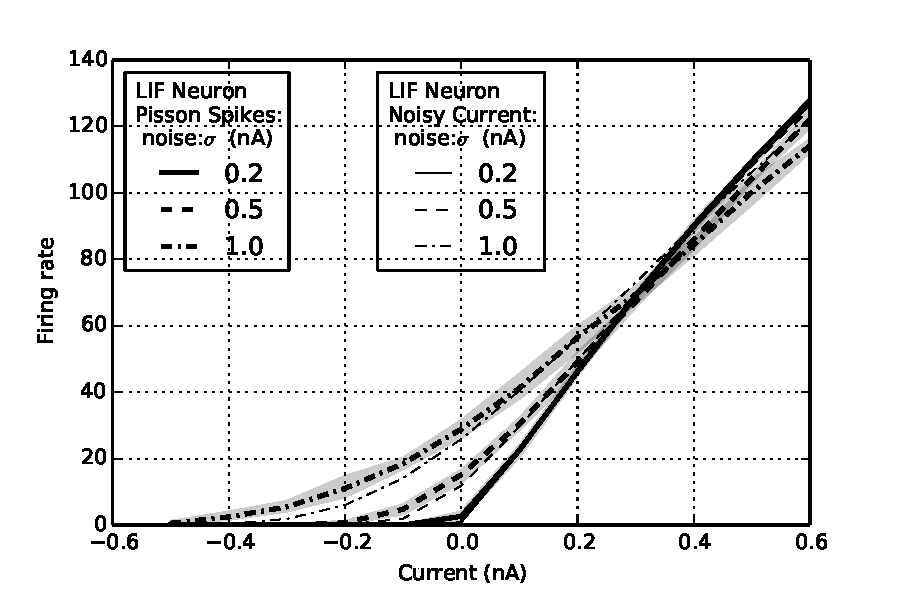
\includegraphics[width=\textwidth]{pics_iconip/3-1.pdf}
%		    \caption{$\tau_m=1$~ms}
%		    \label{Fig:lif_pois1}
%		\end{subfigure}
%		\begin{subfigure}[t]{0.45\textwidth}
%			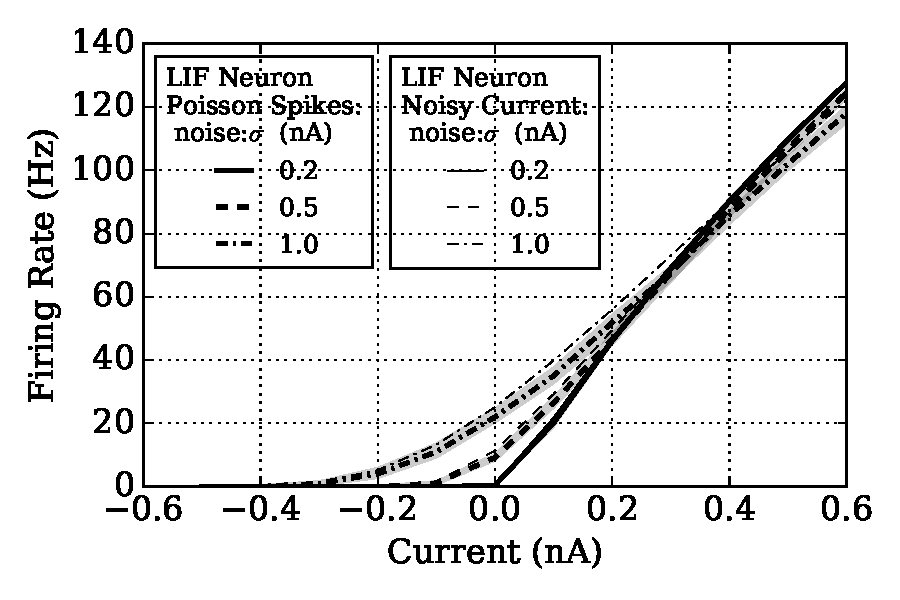
\includegraphics[width=\textwidth]{pics_iconip/3-2.pdf}
%		    \caption{$\tau_m=5$~ms}
%		    \label{Fig:lif_pois5}
%		\end{subfigure}
%		
%		\caption{
%			Recorded response firing rate of two LIF neurons with different synaptic constants.
%			The driving noisy current is simulated with Poission spike trains and the results are compared to the noisy current source.}
%		\label{fig:lif_pois}	
%	\end{figure}
	

	

		
	\subsection{Noisy Softplus}
	Inspired by the set of response functions triggered by different levels of noise, we propose the Noisy Softplus activation function:
	\begin{equation}
	y = f_{ns}(x, \sigma) = k \sigma \log [1 + \exp(\frac{x}{k \sigma})],
	\label{equ:nsp}
	\end{equation}
	where $x$ refers to the mean current, $y$ is the normalised output firing rate, $\sigma$ plays an important role to define the noise level, and $k$, which is determined by the neuron parameters, controls the curve scaling.
	Note that the novel activation function we propose contains two parameters, the current and its noise; both are naturally obtained in spiking neurons.
	% With doubled information, more powerful training methods and network models are expected. 
	Figures~\ref{Fig:nsp} and~\ref{Fig:3d} show the activation function in curve sets and in a 3D plot.
	\begin{figure}[htb!]
		\centering
		\begin{subfigure}[t]{0.6\textwidth}
			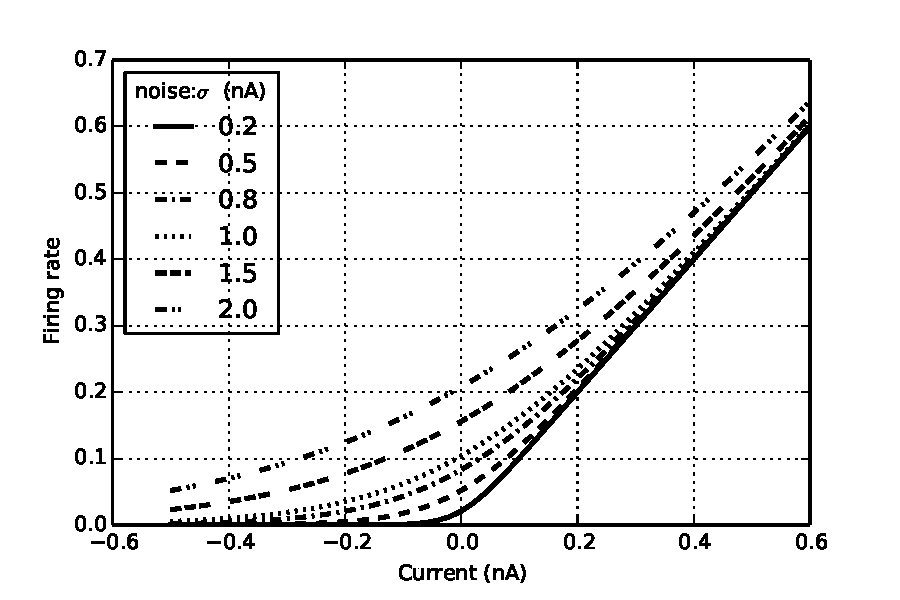
\includegraphics[width=\textwidth]{pics_iconip/4.pdf}
			\caption{Noisy Softplus}
			\label{Fig:nsp}
		\end{subfigure}\\
		\begin{subfigure}[t]{0.6\textwidth}
			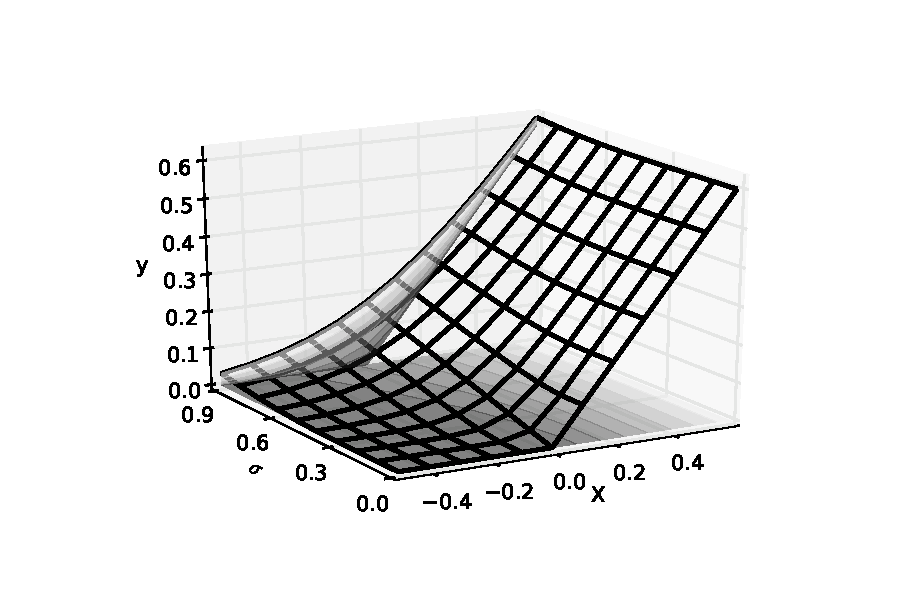
\includegraphics[width=\textwidth]{pics_iconip/5.pdf}
			\caption{Noisy Softplus in 3D}
			\label{Fig:3d}
		\end{subfigure}
		\caption{
			Noisy Softplus fits to the response function of the LIF neuron.
			Noisy Softplus in (a) curve sets and (b) 3D.}
		\label{fig:nsp}
	\end{figure}	
	
	
	The Noisy Softplus fits well to the recorded response firing rate of the LIF neuron with suitable calibration of $k$, see Figure~\ref{Fig:nsptau1}.
	
	\begin{figure}
		\centering
		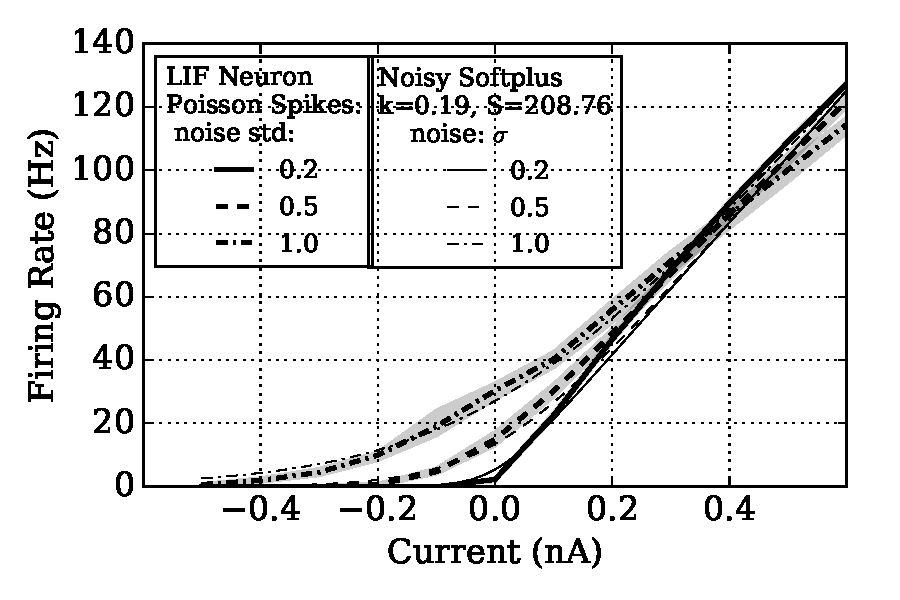
\includegraphics[width=0.6\textwidth]{pics_iconip/4-1.pdf}
		\caption{Noisy Softplus fits to the response firing rates of LIF neurons.}
		\label{Fig:nsptau1}
	\end{figure}		
	
	The derivative is the logistic function scaled by $k\sigma$:
	\begin{equation}
	\frac{\partial f_{ns}(x,\sigma)}{\partial x} = \frac{1}{1+exp(-\frac{x}{k\sigma})}.
	\label{equ:logist}
	\end{equation}	
	
	\begin{figure}[bt!]
		\centering
		\begin{subfigure}[t]{0.3\textwidth}
			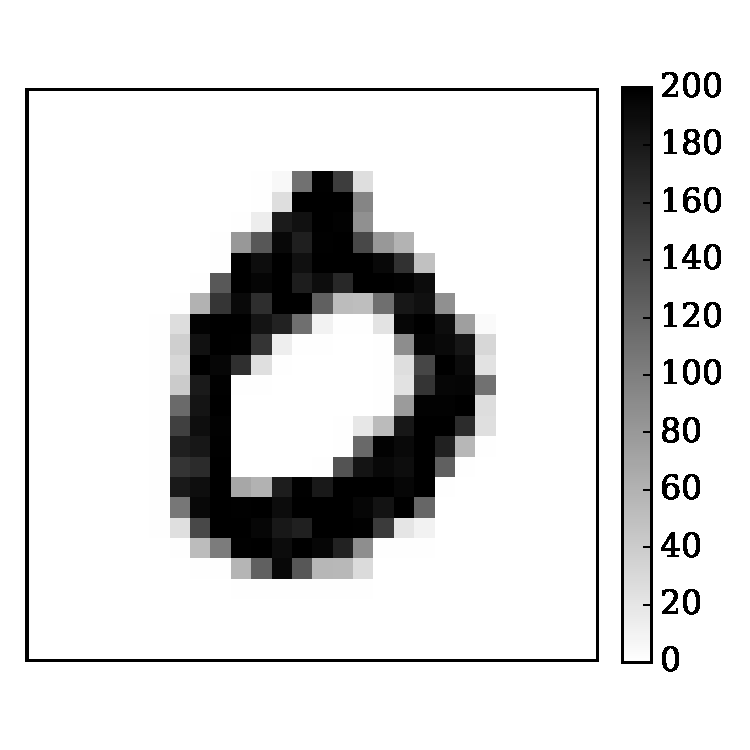
\includegraphics[width=\textwidth]{pics_iconip/6-2.pdf}
		    \caption{Pixel firing rates}
		    \label{Fig:62}
		\end{subfigure}
		\begin{subfigure}[t]{0.3\textwidth}
			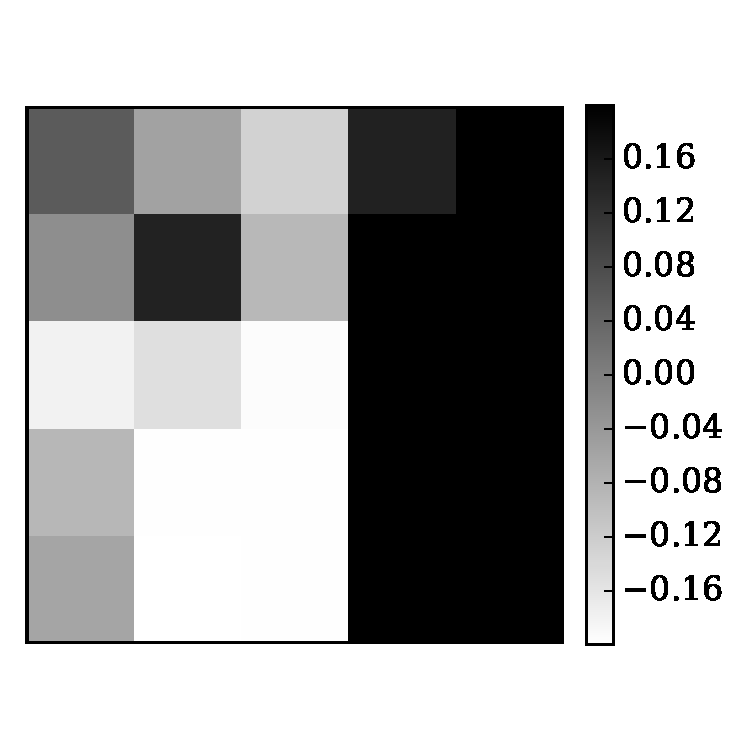
\includegraphics[width=\textwidth]{pics_iconip/6-3.pdf}
		    \caption{5x5 kernel}
		    \label{Fig:63}
		\end{subfigure}
		\begin{subfigure}[t]{0.3\textwidth}
			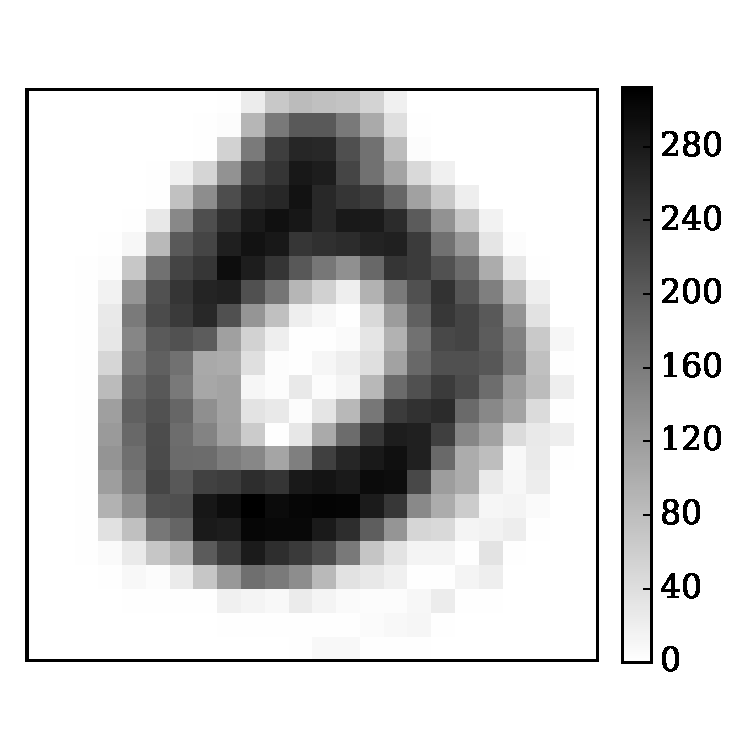
\includegraphics[width=\textwidth]{pics_iconip/6-4.pdf}
		    \caption{Output firing rates}
		    \label{Fig:64}
		\end{subfigure}
		\\
		\begin{subfigure}[t]{0.4\textwidth}
			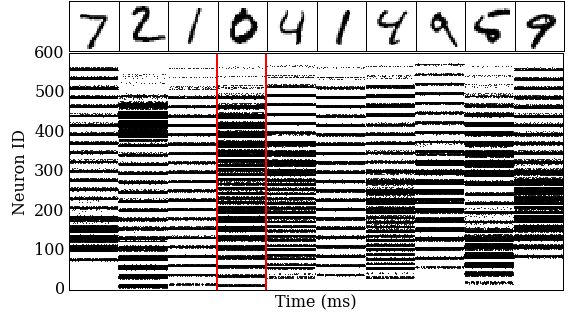
\includegraphics[width=\textwidth]{pics_iconip/6-1.png}
		    \caption{10 input digits as a raster plot}
		    \label{Fig:61}
		\end{subfigure}
		\begin{subfigure}[t]{0.4\textwidth}
			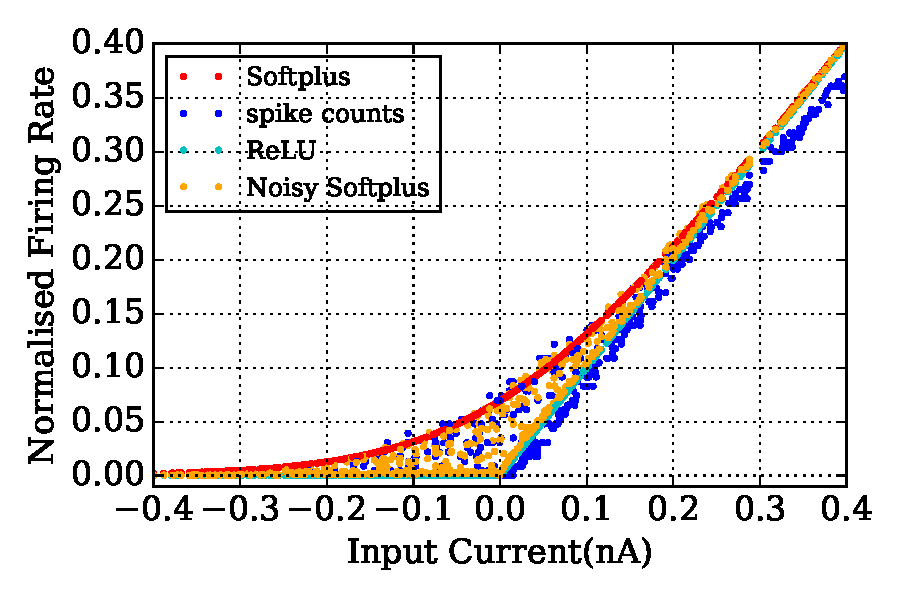
\includegraphics[width=\textwidth]{pics_iconip/6-5.pdf}
		    \caption{Observed `activation functions'}
		    \label{Fig:65}
		\end{subfigure}
		\caption{
			Noisy Softplus fits to the neural response firing rate in an SNN simulation.
			The 28x28 Poisson spike trains in (a) firing rate, and (d) raster plots, are convolved with a 5x5 kernel (b).
			(c) the convolved map with the firing rates of each neuron.
			(e) the normalised firing rate compared with Noisy Softplus, Softplus and ReLU activation functions.}
		\label{fig:cnn}
	\end{figure}
\section{Results}
	A ConvNet model was trained on MNIST,
	%	~\cite{lecun1998gradient}
	a popular database in neuromorphic vision, using Noisy Softplus neurons.
	The architecture contains 28x28 input units, followed by two convolutional layers c5-2s-12c5-2s, and the 10 output neurons represents the classified digit.
	All the convolution and average sampling neurons use Noisy Softplus units with no bias, while the output neurons are softmax units converting a vector of values into the range (0, 1) that add up to 1.
	The weights were updated using a fixed learning rate, 50 images per batch and 10 epochs.
	Before testing on spiking LIF neurons, the weights of each layer were scaled to ensure that input synaptic currents stay within a valid range.
	
	To validate how well the Noisy Softplus activation fits to the response firing rate of LIF neurons in a real application, we simulated the model on Nest using the Poisson MNIST dataset~\cite{liu2016bench} and the neurons of a convolutional map were observed.
	Figure~\ref{fig:cnn} shows the convolution of a 5x5 kernel with an input digit `0' represented by spike trains.
	The estimated spike counts using Noisy Softplus fit to the real recorded firing rate much more accurately than the Softplus and ReLU activation functions.
	In Figure~\subref*{Fig:65}, we manually selected a suitable scaling factor for Softplus which located on the top slope of the response activity.
	However, the scale factor remains static for all the neurons, thus resulting in a mismatch at different level of noise.
	Noisy Softplus adapts to noise automatically.
	
	
	
	
	We compared the training using ReLU, Softplus, and Noisy Softplus by their loss during training averaged over 6 trials, see Figure\ref{fig:training}.
	The trained networks were scaled to SNNs and compared on recognition rates, 93.34\%, 96.43\% and 97.03\% with a conversion loss of 4.76\%, 0.91\% and 0.74\%.
	As it is a major concern in neuromorphic vision, the recognition performance over short response times is also estimated in Figure~\ref{Fig:response}.
	\begin{figure}[bt!]
		\centering
		\begin{subfigure}[t]{0.6\textwidth}
			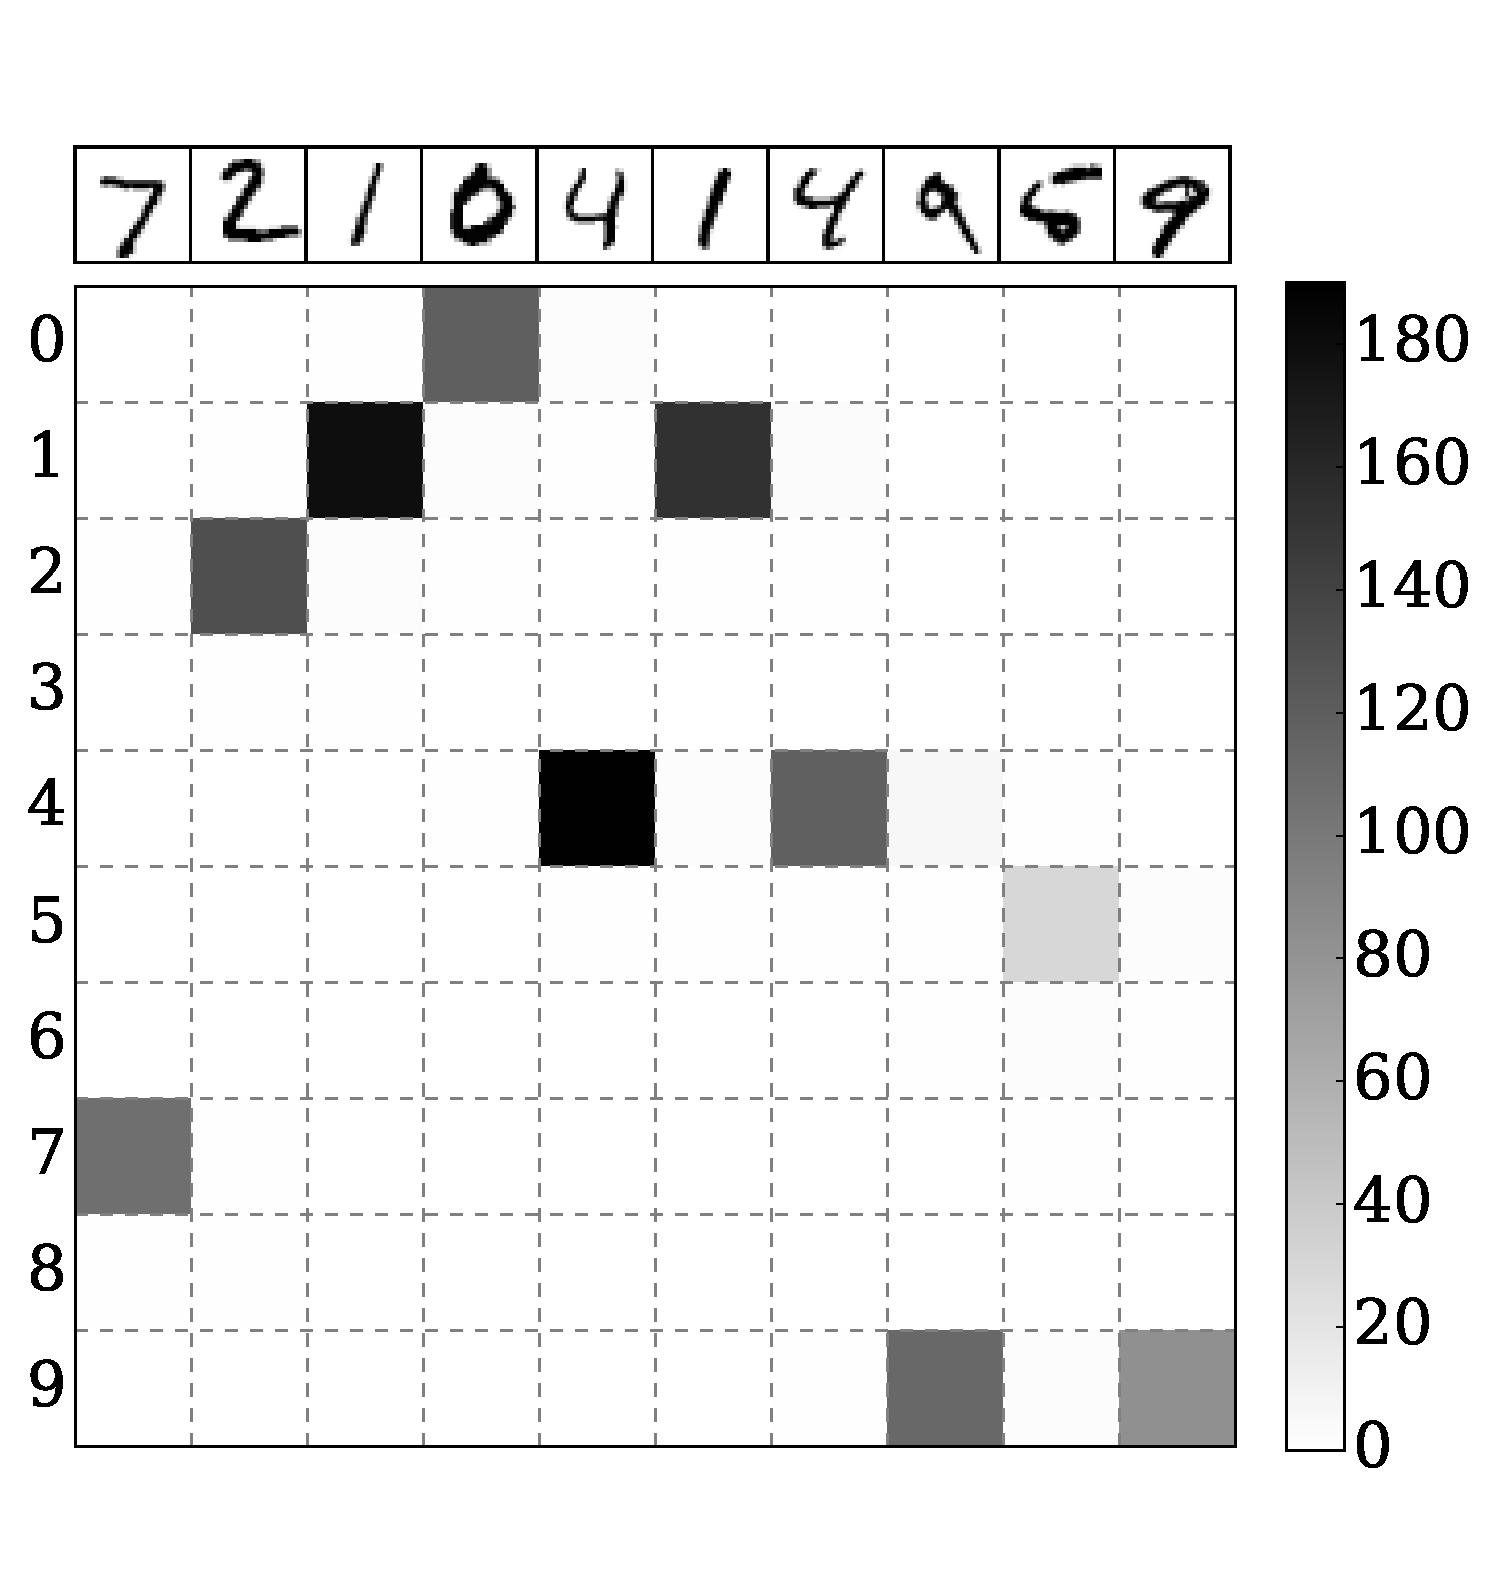
\includegraphics[width=\textwidth]{pics_iconip/7.pdf}
		    \caption{Output firing rates}
		    \label{Fig:out}
		\end{subfigure}
		\\
		\begin{subfigure}[t]{0.7\textwidth}
			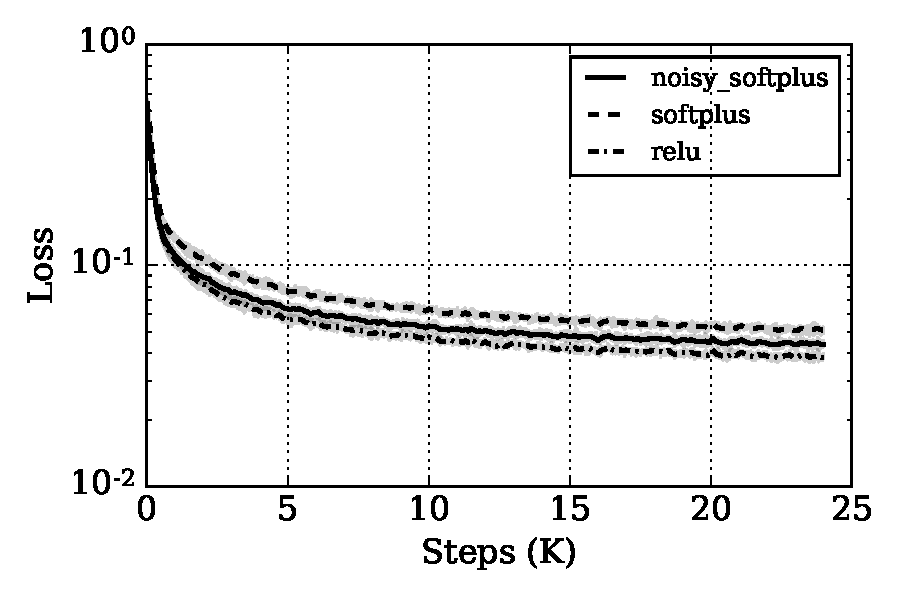
\includegraphics[width=\textwidth]{pics_iconip/8.pdf}
		    \caption{Loss over training}
		    \label{Fig:loss}
		\end{subfigure}\\
		\begin{subfigure}[t]{0.7\textwidth}
			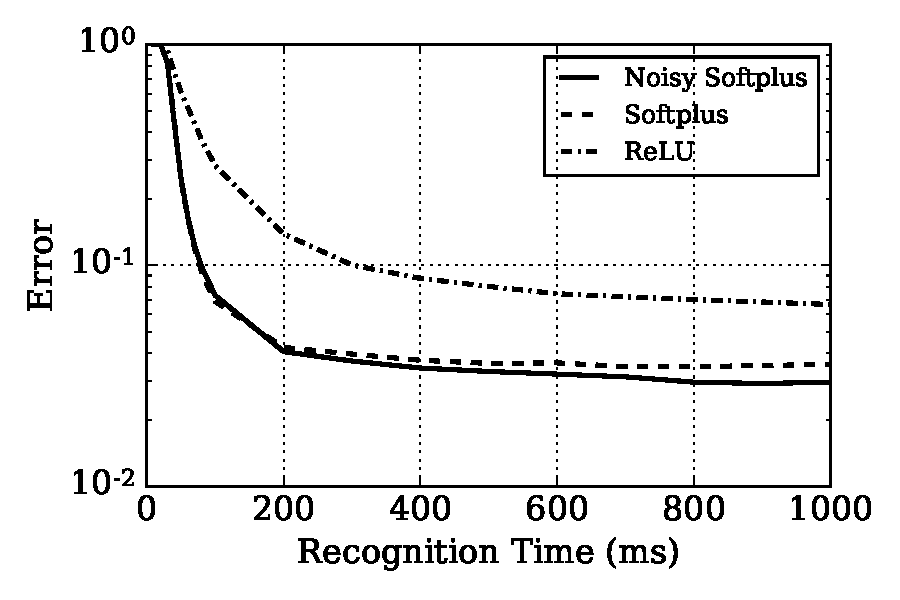
\includegraphics[width=\textwidth]{pics_iconip/9.pdf}
		    \caption{Performance over time}
		    \label{Fig:response}
		\end{subfigure}

		\caption{
			Classification performance is calculated by the firing rate of output neurons (a).
			(b) shows how the loss varies over training.
			(c) illustrates the accuracy over short response times.}
		\label{fig:training}	
	\end{figure}
\section{Summery}
	The Spiking Neural Network (SNN) has not achieved the recognition/classification performance of its non-spiking competitor, the Artificial Neural Network(ANN), particularly when used in deep neural networks.
	How to equip SNNs with equivalent recognition capability as DNNs' thus to take advantages of their neuromorphic implementation attracts increased attention both in the neuromorphic community and the deep learning industry.
	%TODO the scalability, power efficiency and real-time sensor interactive with the environment 
	%	The mapping of a well-trained ANN to an SNN is a hot topic in this field, especially using spiking neurons with biological characteristics.
	This Chapter proposes a new biologically-inspired activation function, Noisy Softplus, which is well-matched to the response function of LIF (Leaky Integrate-and-Fire) neurons.
	A convolutional network (ConvNet) was trained on the MNIST database with Noisy Softplus units and converted to an SNN while maintaining a close classification accuracy.
	This result demonstrates the equivalent recognition capability of the more biologically-realistic SNNs and bring biological features to the activation units in ANNs.
	
	The biologically-inspired activation function, Noisy Softplus, adapts to the noise level of input currents automatically, and is the first attempt to map activation units accurately to the firing response of LIF neurons.
	Noisy Softplus not only brings more biological features to the activation function, but also proves capable of performing well in a spiking ConvNet recognition task.
	The spiking version of Noisy Softplus wins on accuracy over the sigmoid neuron, compared to the result~\cite{Stromatias2015scalable} of using Siegert units.
	As a result of its more accurate mapping, Noisy Softplus outperforms Softplus.
	
	The Noisy Softplus activation function proposed here is based on LIF neurons with biological characteristics, and is the first attempt to map a spiking neural response accurately to the activation unit of an ANN.
	The resulting classification accuracy was tested on a spiking ConvNet; the performance was close to that of the original ConvNet, and was better than using Softplus.
	This study brings a significant biological feature, noise, to the activation units of an ANN, in the hope of promoting research into noise-based computation.
	
	Future work on SNNs will include constraints during training to limit the function within the active range, which is equivalent to constraining the maximum firing rate of an LIF neuron.
	As a result there should be no need for the scaling process after training.
	For more accurate mapping, the scale factor $k$ should be (numerically) derived to avoid calibration.
	In ANNs, it could be useful to study noise as extra information to be gathered by Softplus activation to enhance classification.